\documentclass[a4paper]{article}

\input{style/ch_xelatex.tex}
\input{style/scala.tex}

\graphicspath{ {images/} }
\usepackage{ctex}
\usepackage{graphicx}
\usepackage{color,framed}%文本框
\usepackage{listings}
\usepackage{caption}

\usepackage{hyperref}
\hypersetup{hidelinks,
	colorlinks=true,
	allcolors=black,
	pdfstartview=Fit,
	breaklinks=true}


\usepackage{amssymb}
\usepackage{enumerate}
\usepackage{xcolor}
\usepackage{bm} 
\usepackage{lastpage}%获得总页数
\usepackage{fancyhdr}
\usepackage{tabularx}  
\usepackage{geometry}
\usepackage{minted}
\usepackage{graphics}
\usepackage{subfigure}
\usepackage{float}
\usepackage{pdfpages}
\usepackage{pgfplots}
\pgfplotsset{width=10cm,compat=1.9}
\usepackage{multirow}
\usepackage{footnote}
\usepackage{booktabs}
\usepackage{listings}

%-----------------------伪代码------------------
\usepackage{algorithm}  
\usepackage{algorithmicx}  
\usepackage{algpseudocode}  
\floatname{algorithm}{Algorithm}  
\renewcommand{\algorithmicrequire}{\textbf{Input:}}  
\renewcommand{\algorithmicensure}{\textbf{Output:}} 
\usepackage{lipsum}  
\makeatletter
\newenvironment{breakablealgorithm}
  {% \begin{breakablealgorithm}
  \begin{center}
     \refstepcounter{algorithm}% New algorithm
     \hrule height.8pt depth0pt \kern2pt% \@fs@pre for \@fs@ruled
     \renewcommand{\caption}[2][\relax]{% Make a new \caption
      {\raggedright\textbf{\ALG@name~\thealgorithm} ##2\par}%
      \ifx\relax##1\relax % #1 is \relax
         \addcontentsline{loa}{algorithm}{\protect\numberline{\thealgorithm}##2}%
      \else % #1 is not \relax
         \addcontentsline{loa}{algorithm}{\protect\numberline{\thealgorithm}##1}%
      \fi
      \kern2pt\hrule\kern2pt
     }
  }{% \end{breakablealgorithm}
     \kern2pt\hrule\relax% \@fs@post for \@fs@ruled
  \end{center}
  }
\makeatother
%------------------------代码-------------------
\RequirePackage{listings}
\RequirePackage{xcolor}
\definecolor{dkgreen}{rgb}{0,0.6,0}
\definecolor{gray}{rgb}{0.5,0.5,0.5}
\definecolor{mauve}{rgb}{0.58,0,0.82}
\lstset{
	numbers=left,  
	frame=tb,
	aboveskip=3mm,
	belowskip=3mm,
	showstringspaces=false,
	columns=flexible,
	framerule=1pt,
	rulecolor=\color{gray!35},
	backgroundcolor=\color{gray!5},
	basicstyle={\ttfamily},
	numberstyle=\tiny\color{gray},
	keywordstyle=\color{blue},
	commentstyle=\color{dkgreen},
	stringstyle=\color{mauve},
	breaklines=true,
	breakatwhitespace=true,
	tabsize=3,
}

%-------------------------页面边距--------------
\geometry{a4paper,left=2.3cm,right=2.3cm,top=2.7cm,bottom=2.7cm}
%-------------------------页眉页脚--------------
\usepackage{fancyhdr}
\pagestyle{fancy}
\lhead{\kaishu 数据安全课程作业}
\chead{秘密共享实践}
\rhead{2211044 {\CJKfontspec{simkai.ttf} 陆皓喆}}%加粗\bfseries 
\lfoot{}
\cfoot{\thepage}
\rfoot{}
\renewcommand{\headrulewidth}{0.1pt}  
\renewcommand{\footrulewidth}{0pt}%去掉横线
\newcommand{\HRule}{\rule{\linewidth}{0.5mm}}%标题横线
\newcommand{\HRulegrossa}{\rule{\linewidth}{1.2mm}}
\setlength{\textfloatsep}{10mm}%设置图片的前后间距
%--------------------文档内容--------------------

\begin{document}
\renewcommand{\contentsname}{目\ 录}
\renewcommand{\appendixname}{附录}
\renewcommand{\appendixpagename}{附录}
\renewcommand{\refname}{参考文献} 
\renewcommand{\figurename}{图}
\renewcommand{\tablename}{表}
\renewcommand{\today}{\number\year 年 \number\month 月 \number\day 日}

%-------------------------封面----------------
\begin{titlepage}
    \begin{center}
    
\includegraphics[width=0.8\textwidth]{NKU.png}\\[1cm]
    \vspace{20mm}
        \textsc{\Huge \kaishu{\textbf{南开大学}} }\\[0.9cm]
        \textsc{\huge \kaishu{\textbf{计算机学院和密码与网络空间安全学院}}}\\[0.9cm]
        \textsc{\Large \textbf{《数据安全》课程作业}}\\[0.8cm]
        \HRule \\[0.9cm]
        { \LARGE \bfseries 秘密共享实践}\\[0.4cm]
        \HRule \\[2.0cm]

    \vspace{\fill}

    \centering
    \textsc{\LARGE \kaishu{姓名\ :\ {{\CJKfontspec{simkai.ttf} 周重天}}}}\\[0.5cm]
    \textsc{\LARGE \kaishu{学号\ :\ 2311082}}\\[0.5cm]
    \textsc{\LARGE \kaishu{专业\ :\ 计算机科学与技术}}\\[0.5cm]
    
    \vfill
    {\Large \today}
    \end{center}
\end{titlepage}

\renewcommand {\thefigure}{\thesection{}.\arabic{figure}}%图片按章标号
\renewcommand{\figurename}{图}
\renewcommand{\contentsname}{目录}  
\cfoot{\thepage\ of \pageref{LastPage}}%当前页 of 总页数


\newpage
\tableofcontents

\newpage
\section{实验要求}
假设有三个同学需要对班里的优秀干部 Alice、Bob、Charles、Douglas 进行投票，最后统计各个班干部获得的票数。这个时候就可以利用 Shamir 秘密共享将各个投票方的投票分享出去并进行隐私求和计算。

\textbf{借鉴实验3.2，实现三个人对于他们拥有的数据的平均值的计算。}


\section{实验原理}
\subsection{秘密共享}
秘密共享（Secret Sharing）是一种将秘密分割存储的密码技术，目的是阻止秘密过于集中，以达到分散风险和容忍入侵的目的，是信息安全和数据保密中的重要手段。目前，秘密共享已成为一种重要密码学工具，在诸多多方安全计算协议中被使用，例如拜占庭协议、多方隐私集合求交协议、阈值密码学等。 

基于秘密分配和运算的形式，我们将秘密共享分为基于位运算的加性秘密共享和基于线性代数的线性秘密共享。
依据秘密重构的条件或者秘密分享的份额数量等，又可以将秘密共享分为如下类别：
\begin{itemize}
    \item \textbf{门限秘密共享：}任意大于等于阈值的参与方集合可重构出秘密；
    \item \textbf{多重秘密共享：}参与方的子秘密可以多次使用，分别恢复多个共享秘密；
    \item \textbf{多秘密共享：}一次共享，共享多个秘密，且子秘密可以重复使用；
    \item \textbf{可验证秘密共享：}可通过公共变量验证自己子秘密的正确性；
    \item \textbf{动态秘密共享：}允许添加或删除参与方，定期或不定期更新参与方的子秘密，还允许在不同的时间恢复不同的秘密。 
\end{itemize}

\subsection{门限秘密共享}
门限秘密共享（Threshold Secret Sharing）是一种密码学技术，可以将秘密分割成多个部分，并将这些部分分配给不同的参与者，从而保护秘密免受单点故障和恶意攻击。

在门限秘密共享中，将秘密分成$n$个部分，其中只要$k$个部分被收集，就可以重构出原始秘密。这个$k$值称为“门限”，通常满足$k\le n$，以确保秘密不被泄露。只有在收集到至少$k$个部分时，才能重构出秘密，因此，即使一些部分被泄露或丢失，也可以保持秘密的安全性。

门限秘密共享可以用于许多场景，例如：多方拥有的敏感信息（例如金融账户密码）、公共密钥基础设施、加密密钥管理等等。
\begin{figure}[H]
    \centering
    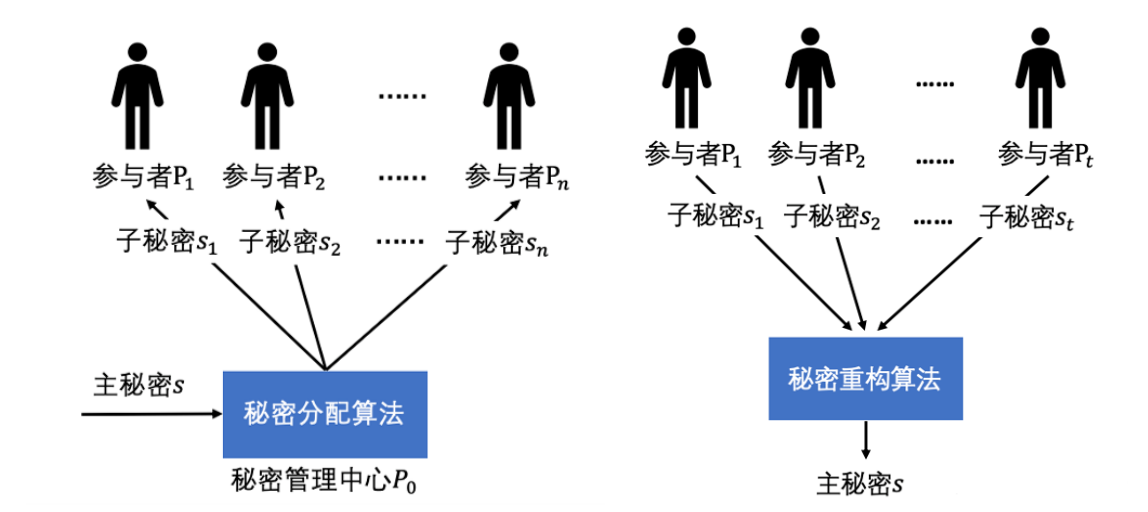
\includegraphics[width=0.75\linewidth]{figure/门限秘密共享实验原理.png}
    \caption{门限秘密共享实验原理}
    \label{fig:enter-label}
\end{figure}

\subsection{基于Shamir门限秘密共享的协议设计}
首先，要基于Shamir门限秘密共享进行协议设计。

以计算Alice的票数为例，三个同学的隐私输入为0或1，0表示不投票给Alice，1表示投票给Alice。假设三个同学$Student_1$、$Student_2$和$Student_3$分别拥有隐私输入a、b和c，他们将各自的隐私输入通过(2,3)门限的Shamir秘密共享分享给另外两个同学：$Student_1$获得a、b和c的秘密份额$a_1$、$b_1$和$c_1$；$Student_2$获得秘密份额$a_2$、$b_2$和$c_2$；$Student_3$获得秘密份额$a_3$、$b_3$和$c_3$。之后，三位同学各自将获得的秘密份额相加，分别得到$d_1=a_1+b_1+c_1$，$d_2=a_2+b_2+c_2$和$d_3=a_3+b_3+c_3$。一个计票员从三个同学中任选两个，例如$Student_2$和$Student_3$，获得他们拥有的$d_2$和$d_3$，就可以重构出$d=a+b+c$，也就是Alice获得的票数总和。
\begin{figure}[H]
    \centering
    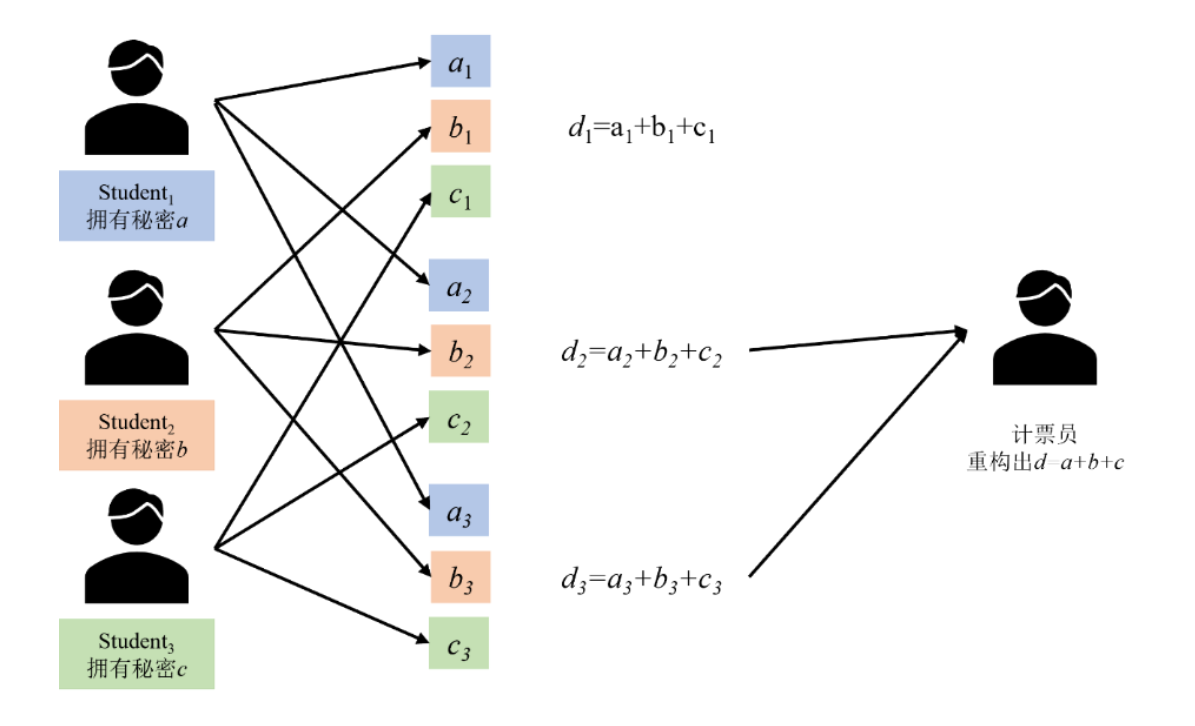
\includegraphics[width=0.75\linewidth]{figure/实验具体原理.png}
    \caption{实验具体原理}
    \label{fig:enter-label}
\end{figure}

\section{实验环境}
本次实验在本机的macos上完成，仅涉及到python及相关环境包。


\section{实验过程}
首先，我们在Lab4目录下新建一个文件夹vote，在vote文件夹下打开终端，分别输入以下命令行：
\begin{minted}[frame=single, linenos=true,breaklines, breakanywhere]{c}
touch ss_function.py
touch ss_student.py
touch count_student.py
touch vote_counter.py
\end{minted}

执行完毕后，如下所示，我们成功新建了四个python文件。
\begin{figure}[H]
    \centering
    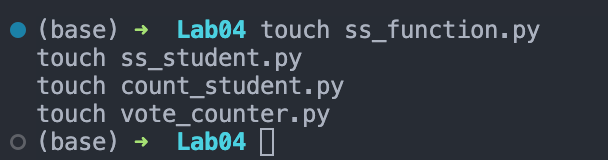
\includegraphics[width=1\linewidth]{figure/新建四个文件.png}
    \caption{新建四个文件}
    \label{fig:enter-label}
\end{figure}

然后，将如下代码复制到 ss\_function.py，ss\_function.py 代码中定义了一些秘密共享过程中三个学生以及计票员会用到的函数。

具体代码如下所示：
\begin{minted}[frame=single, linenos=true,breaklines, breakanywhere]{python}
import random

#快速幂计算 a^b%p
def quickpower(a,b,p):
    a=a%p
    ans=1
    while b!=0:
        if b&1:
            ans=(ans*a)%p
        b>>=1
        a=(a*a)%p
    return ans

#构建多项式：x0 为常数项系数，T 为最高次项次数，p 为模数,fname 为多项式名
def get_polynomial(x0,T,p,fname):
    f=[]
    f.append(x0)
    for i in range(0,T):
        f.append(random.randrange(0,p))
    #输出多项式
    f_print='f'+fname+'='+str(f[0])
    for i in range(1,T+1):
        f_print+='+'+str(f[i])+'x^'+str(i)
    print(f_print)
    return f

#计算多项式值
def count_polynomial(f,x,p):
    ans=f[0]
    for i in range(1,len(f)):
        ans=(ans+f[i]*quickpower(x,i,p))%p
    return ans

#重构函数 f 并返回 f(0)
def restructure_polynomial(x,fx,t,p):
    ans=0
    #利用多项式插值法计算出 x=0 时多项式的值
    for i in range(0,t):
        fx[i]=fx[i]%p
        fxi=1
        #在模 p 下，(a/b)%p=(a*c)%p，其中 c 为 b 在模 p 下的逆元，c=b^(p-2)%p
        for j in range(0,t):
            if j !=i:
                fxi=(-1*fxi*x[j]*quickpower(x[i]-x[j],p-2,p))%p
        fxi=(fxi*fx[i])%p
        ans=(ans+fxi)%p
    return ans
\end{minted}


然后将如下代码复制到 ss\_student.py，三个学生分别执行 ss\_student.py，将自己的秘密投票值共享给另外两个学生。

具体代码如下所示：
\begin{minted}[frame=single, linenos=true,breaklines, breakanywhere]{python}
import ss_function as ss_f
#设置模数 p
p=1000000007
print(f'模数 p：{p}')
#输入参与方 id 以及秘密 s 
id=int(input("请输入参与方 id:"))
s=int(input(f'请输入 student_{id}的投票值 s:'))
#秘密份额为(share_x,share_y)
shares_x=[1,2,3]
shares_y=[]
#计算多项式及秘密份额(t=2,n=3)
print(f'Student_{id}的投票值的多项式及秘密份额：')
f=ss_f.get_polynomial(s,1,p,str(id))
temp=[]
for j in range(0,3):
    temp.append(ss_f.count_polynomial(f,shares_x[j],p))
    print(f'({shares_x[j]},{temp[j]})')
    shares_y.append(temp[j])
#Student_id 将自己的投票值的秘密份额分享给两外两个学生
#将三份秘密份额分别保存到 student_id_1.txt,student_id_2.txt,student_id_3.txt
#Student_i 获得 Student_id_i.txt
for i in range(1,4):
    with open(f'student_{id}_{i}.txt','w') as f:
        f.write(str(shares_y[i-1]))
\end{minted}


然后在命令行执行下面的命令：
\begin{minted}[frame=single, linenos=true,breaklines, breakanywhere]{c}
python3 ss_student.py
1
0
python3 ss_student.py
2
1
python3 ss_student.py
3
0
\end{minted}

结果如下所示：
\begin{figure}[H]
    \centering
    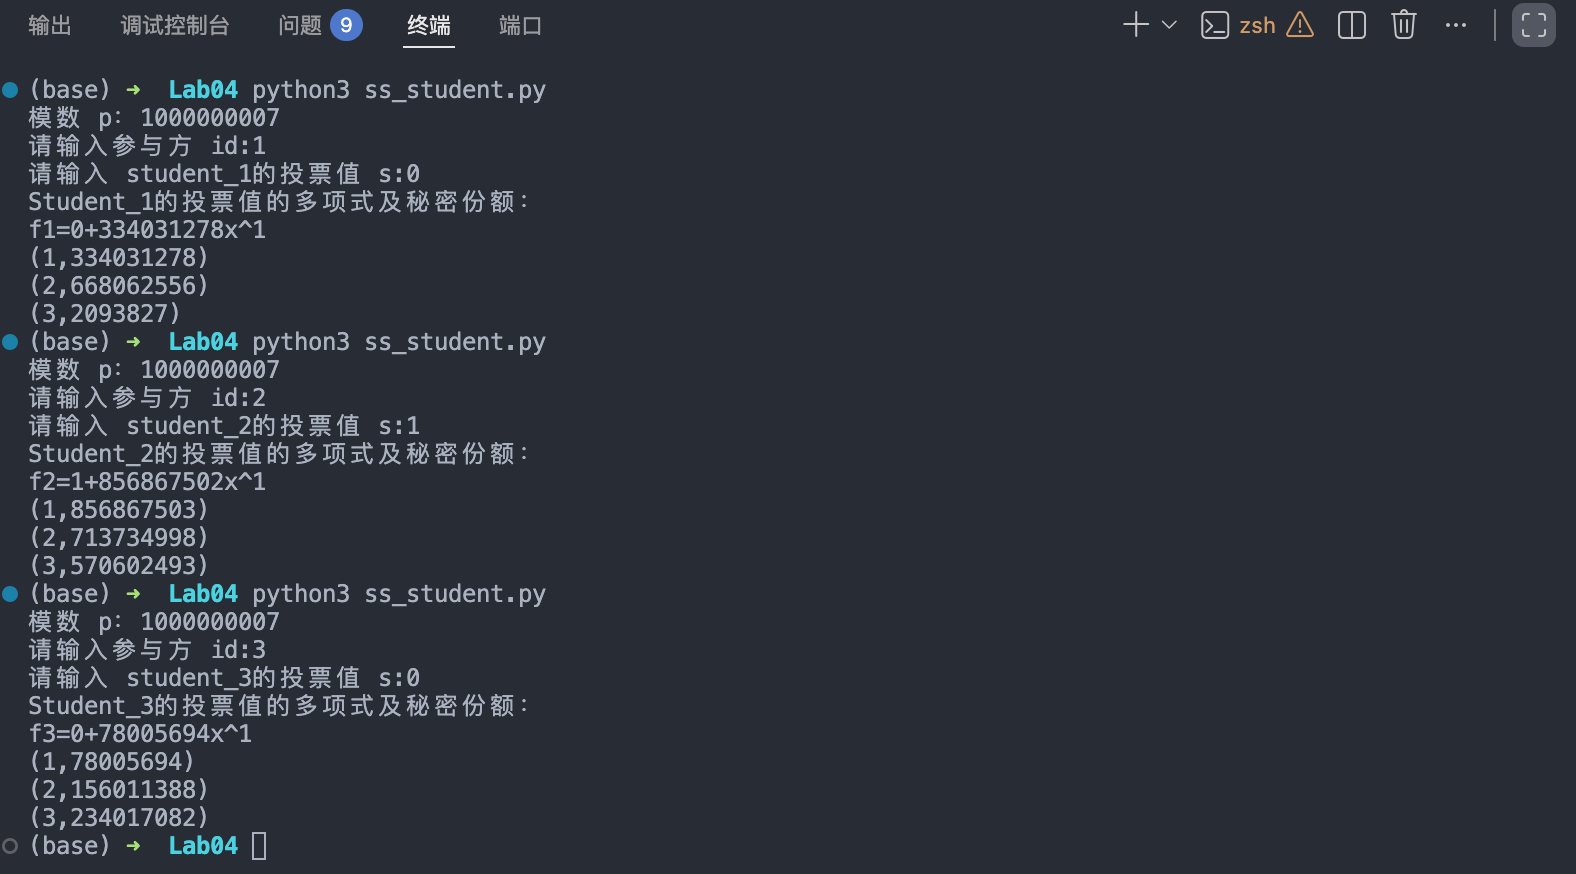
\includegraphics[width=1\linewidth]{figure/student_exec.png}
    \caption{执行ss\_student.py}
    \label{fig:enter-label}
\end{figure}

回到资源管理器，我们可以看到，\textbf{lab04的文件夹下已经生成9个txt文件，分别保存三个秘密值的秘密份额。}
\begin{figure}[H]
    \centering
    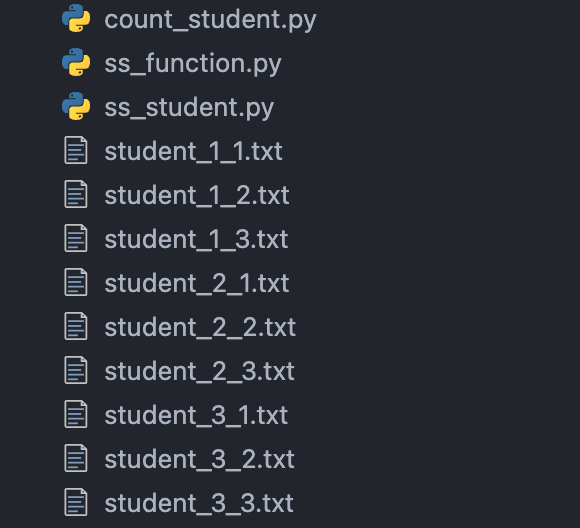
\includegraphics[width=0.75\linewidth]{figure/生成九个文件.png}
    \caption{生成九个文件}
    \label{fig:enter-label}
\end{figure}

然后，将以下代码复制到 count\_student.py，三个学生分别执行 count\_student.py，获取另外两个学生的投票值的秘密份额，并将三个投票值的秘密份额相加。

具体代码如下所示：
\begin{minted}[frame=single, linenos=true,breaklines, breakanywhere]{python}
p=1000000007
#输入参与方 id
id=int(input("请输入参与方 id:"))
#Student_id 读取属于自己的秘密份额student_1_id.txt,student_2_id.txt,student_3_id.txt
data=[]
for i in range(1,4):
    with open(f'student_{i}_{id}.txt', "r") as f: #打开文本
        data.append(int(f.read())) #读取文本
#计算三个秘密份额的和
d=0
for i in range(0,3):
    d=(d+data[i])%p
#将求和后的秘密份额保存到文件 d_id.txt 内
with open(f'd_{id}.txt','w') as f:
    f.write(str(d))
\end{minted}


执行下面三个语句，把三个投票值的秘密份额相加，分别保存到三个文件中。
\begin{minted}[frame=single, linenos=true,breaklines, breakanywhere]{c}
python3 count_student.py
1
python3 count_student.py
2
python3 count_student.py
3
\end{minted}

执行完毕后，结果如下所示：
\begin{figure}[H]
    \centering
    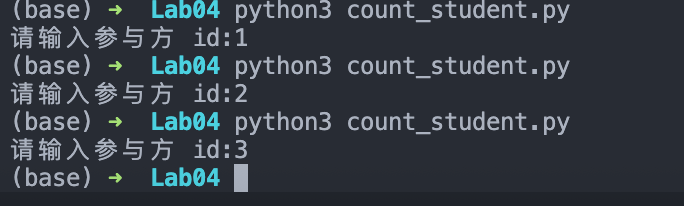
\includegraphics[width=1\linewidth]{figure/执行三个命令完成求和.png}
    \caption{执行三个命令完成求和}
    \label{fig:enter-label}
\end{figure}

结果如下所示，在文件夹 vote 下会产生 3 个 txt 文件，分别为 d\_1.txt、d\_2.txt 和 d\_3.txt。
\begin{figure}[H]
    \centering
    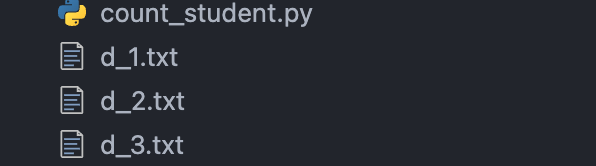
\includegraphics[width=1\linewidth]{figure/生成三个文件.png}
    \caption{执行三个命令完成求和}
    \label{fig:enter-label}
\end{figure}
继续，将以下代码复制到vote\_counter.py，具体代码如下所示：
\begin{minted}[frame=single, linenos=true,breaklines, breakanywhere]{python}
import ss_function as ss_f
#设置模数 p
p=1000000007
#随机选取两个参与方，例如 student2 和 student3，获得 d2,d3，从而恢复出 d=a+b+c
#读取 d2,d3
d_23=[]
for i in range(2,4):
    with open(f'd_{i}.txt', "r") as f: #打开文本
        d_23.append(int(f.read())) #读取文本
#加法重构获得 d
d=ss_f.restructure_polynomial([2,3],d_23,2,p)
# 这一步是为了计算平均值
d = d / 3
print(f'得票结果为：{d}')
\end{minted}


执行命令：
\begin{minted}[frame=single, linenos=true,breaklines, breakanywhere]{c}
python3 vote_counter.py
\end{minted}

结果如下所示：
\begin{figure}[H]
    \centering
    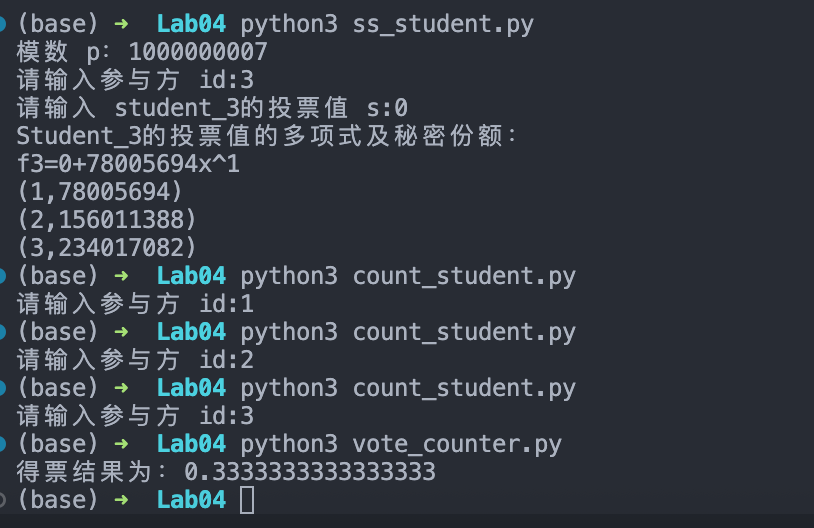
\includegraphics[width=1\linewidth]{figure/计算平均值的结果.png}
    \caption{计算平均值的结果}
    \label{fig:enter-label}
\end{figure}

\textbf{由此可见，三人的原始投票为 0、1、0，计算得到的平均值为 0.333，说明平均值计算正确。}

这样的话，实验就成功了。

\section{实验心得与体会}
通过本次实验，我进一步理解了 Shamir 门限秘密共享在隐私计算中的应用方式。实验中，三位参与方并没有直接公开自己的原始输入，而是先将投票值构造成一次多项式上的秘密份额，再分别分发给其他参与方。随后，各参与方只对自己持有的份额进行本地求和，计票方只需收集其中两个求和后的份额，就可以利用拉格朗日插值恢复出总和，并进一步得到平均值。整个过程体现了秘密共享的线性性质，也说明在不暴露单个参与方隐私数据的情况下，仍然可以完成有效的统计计算。

此外，三人的输入为 $0,1,0$，最终恢复出的平均值为 $0.333$，与理论计算结果一致，说明程序实现是正确的。实验过程中我也认识到，模数的选择、多项式构造、份额生成以及插值重构都是协议正确运行的关键步骤。如果份额读取错误或重构时选取的参与方数量不足，就无法得到正确结果。因此，本次实验不仅加深了我对门限秘密共享原理的理解，也让我体会到密码协议在实际实现中需要同时关注安全性、正确性和工程细节。

\end{document}